\documentclass[leqno,11pt]{article}

\usepackage{graphicx}
\usepackage{subcaption}
\usepackage[margin=1in]{geometry}
\usepackage{float}
\usepackage{hyperref}
\usepackage{cleveref}
\usepackage{booktabs}
\usepackage{longtable}
\usepackage{csvsimple}

\csvset{respect underscore}

\newcommand{\importcsv}[1]{{\scriptsize\setlength{\tabcolsep}{3pt}\csvautobooklongtable{#1}}}

\hypersetup{
  colorlinks=true,
  linkcolor=red,
  filecolor=magenta,
  urlcolor=blue,
}

\graphicspath{{./}{../charts/}{../../analysis/charts/}}

\title{Benchmark Evaluation Charts}
\author{Standalone Figure Compilation}
\date{\today}

\begin{document}

\maketitle

\section{Tuple Flattening}

\subsection{MLton Benchmarks (Tuple Flattening)}

\begin{figure}[H]
  \centering
  \begin{subfigure}[b]{0.32\textwidth}
    \centering
    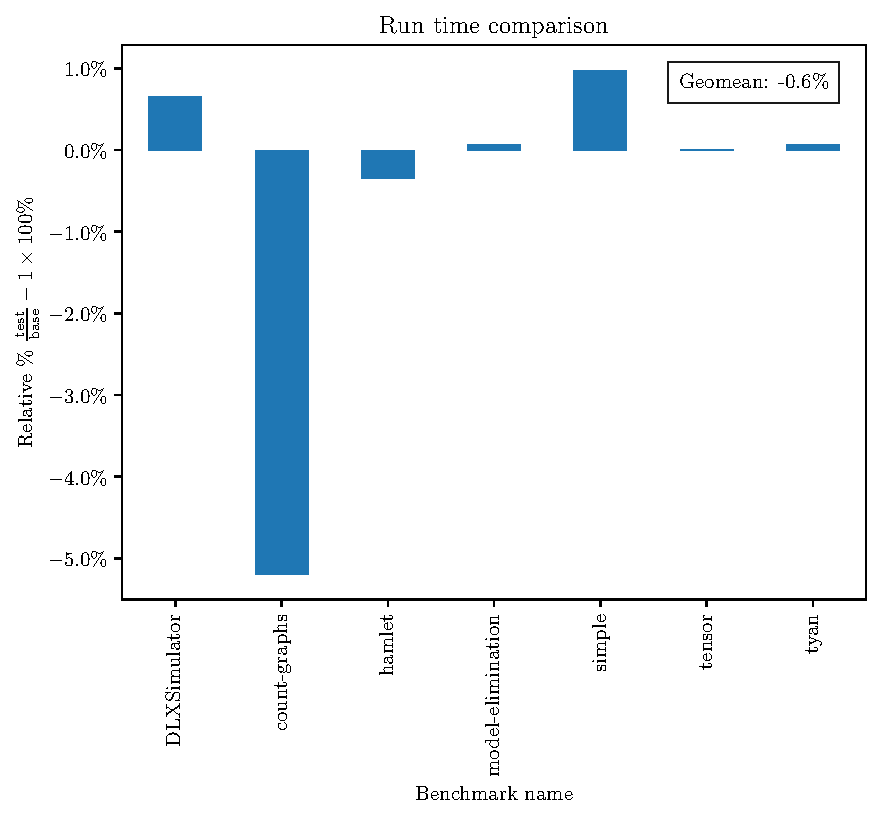
\includegraphics[width=\textwidth]{tuple_mlton_run_mlton_vs_mlton.pdf}
    \caption{Run time}
    \label{fig:tuple_mlton_run_mlton_vs_mlton}
  \end{subfigure}
  \hfill
  \begin{subfigure}[b]{0.32\textwidth}
    \centering
    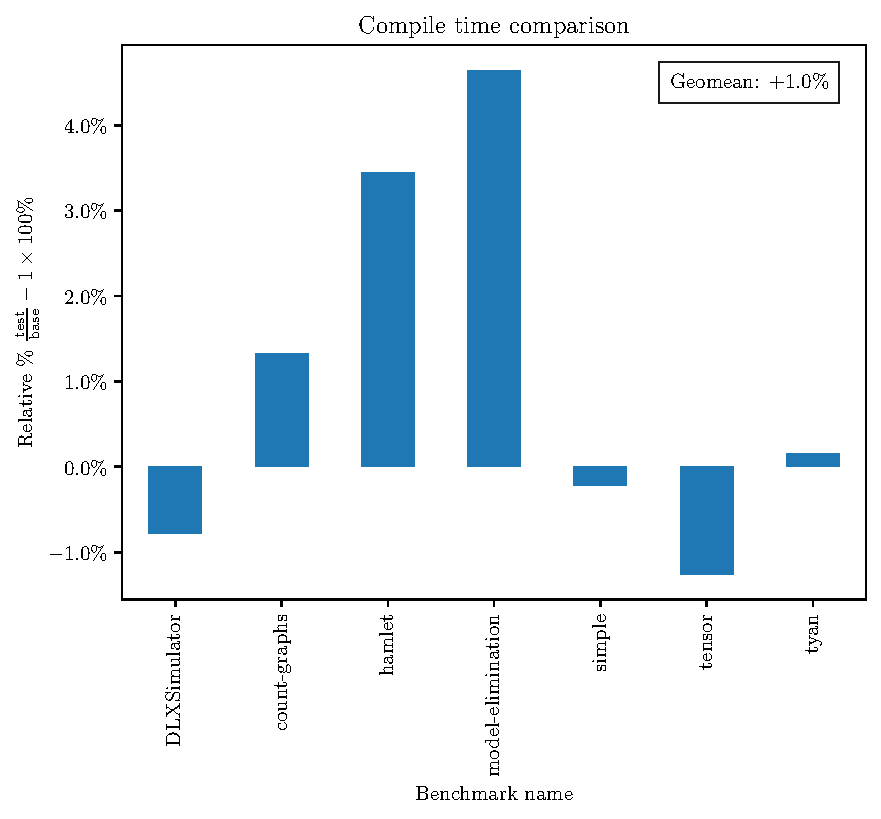
\includegraphics[width=\textwidth]{tuple_mlton_compile_mlton_vs_mlton.pdf}
    \caption{Compile time}
    \label{fig:tuple_mlton_compile_mlton_vs_mlton}
  \end{subfigure}
  \hfill
  \begin{subfigure}[b]{0.32\textwidth}
    \centering
    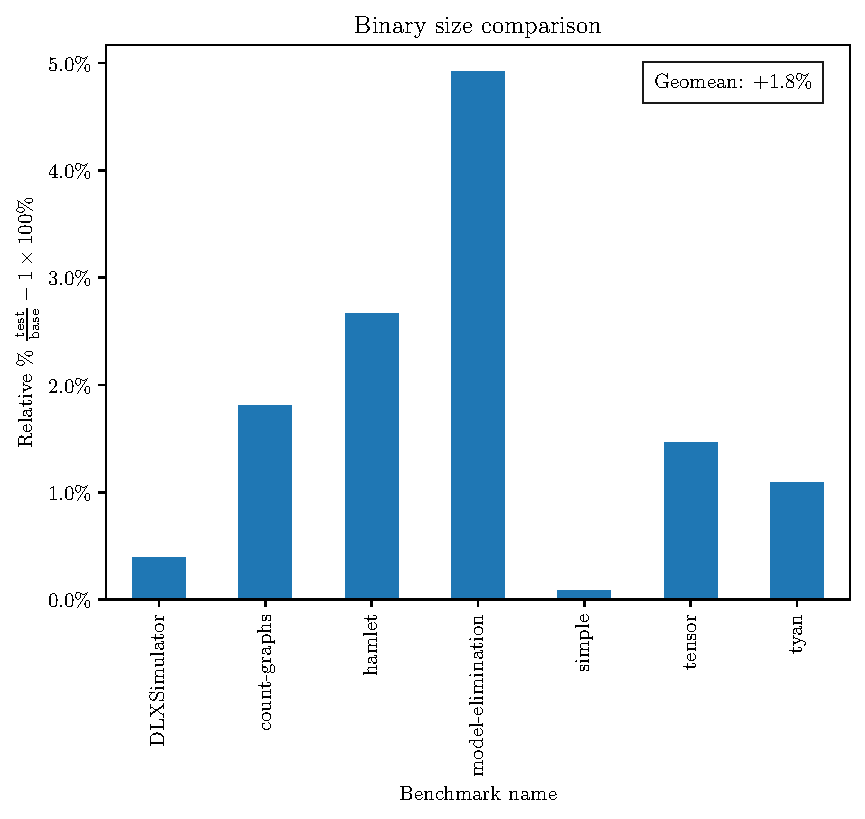
\includegraphics[width=\textwidth]{tuple_mlton_size_mlton_vs_mlton.pdf}
    \caption{Binary size}
    \label{fig:tuple_mlton_size_mlton_vs_mlton}
  \end{subfigure}
  \caption{Relative performance for with- vs without-\texttt{PreFlatten} on the MLton benchmark suite. Data: \protect\nolinkurl{test_tuple_flatten_mlton_mlton_o3:flattening-tests:fd9a06c:20260825_064158.jsonl}. <0\% represents an improvement, >0\% represents a regression.}
  \label{fig:tuple_mlton}
\end{figure}

\subsection{\texttt{parallel-ml-bench}: MLton vs MLton (Tuple Flattening)}

\begin{figure}[H]
  \centering
  \begin{subfigure}[b]{0.48\textwidth}
    \centering
    \includegraphics[width=\textwidth]{tuple_parallel_bench_run_mlton_vs_mlton.pdf}
    \caption{Run time}
    \label{fig:tuple_parallel_bench_run_mlton_vs_mlton}
  \end{subfigure}
  \hfill
  \begin{subfigure}[b]{0.48\textwidth}
    \centering
    \includegraphics[width=\textwidth]{tuple_parallel_bench_size_mlton_vs_mlton.pdf}
    \caption{Binary size}
    \label{fig:tuple_parallel_bench_size_mlton_vs_mlton}
  \end{subfigure}
  \caption{Relative performance for with- vs without-\texttt{PreFlatten}, applied to tuple constructors on the \texttt{parallel-ml-bench} benchmark suite. Data: \protect\nolinkurl{mlton_tuple_mlton_parallel_o3:260825-001542:flattening-tests:dcd9cf195eacea093ebe838dcb1d190333218ffd:260825-001542.processed.jsonl}. <0\% represents an improvement, >0\% represents a regression.}
  \label{fig:tuple_parallel_bench}
\end{figure}

\subsection{\texttt{parallel-ml-bench}: MPL vs MPL (Tuple Flattening)}

\begin{figure}[H]
  \centering
  \begin{subfigure}[b]{0.48\textwidth}
    \centering
    \includegraphics[width=\textwidth]{tuple_parallel_bench_run_mpl_vs_mpl.pdf}
    \caption{Run time}
    \label{fig:tuple_parallel_bench_run_mpl_vs_mpl}
  \end{subfigure}
  \hfill
  \begin{subfigure}[b]{0.48\textwidth}
    \centering
    \includegraphics[width=\textwidth]{tuple_parallel_bench_size_mpl_vs_mpl.pdf}
    \caption{Binary size}
    \label{fig:tuple_parallel_bench_size_mpl_vs_mpl}
  \end{subfigure}
  \caption{Relative performance for with- vs without-\texttt{PreFlatten}, applied to tuple constructors on the \texttt{parallel-ml-bench} benchmark suite, for the MPL compiler, at a variety of core counts. Data: \protect\nolinkurl{mpl_tuple_mpl_parallel_o3_morecores:260825-204258:flattening-tests:475993b514ca4e4f6921a54f390c1ba9bc2350a1:260825-204258.processed.jsonl}. <0\% represents an improvement, >0\% represents a regression.}
  \label{fig:tuple_parallel_bench_mpl}
\end{figure}

\begin{figure}[H]
  \centering
  \includegraphics[width=\textwidth,height=0.88\textheight,keepaspectratio]{tuple_parallel_bench_run_mpl_vs_mpl_geomean.pdf}
  \caption{Relative performance for with- vs without-\texttt{PreFlatten}, applied to tuple constructors on the \texttt{parallel-ml-bench} benchmark suite, for the MPL compiler, at a variety of core counts. Data: \protect\nolinkurl{mpl_tuple_mpl_parallel_o3_morecores:260825-204258:flattening-tests:475993b514ca4e4f6921a54f390c1ba9bc2350a1:260825-204258.processed.jsonl}. <0\% represents an improvement, >0\% represents a regression.}
  \label{fig:tuple_parallel_bench_mpl_geomean}
\end{figure}

\begin{figure}[H]
  \centering
  \includegraphics[width=\textwidth,height=0.88\textheight,keepaspectratio]{tuple_parallel_bench_run_mpl_vs_mpl_trellis.pdf}
  \caption{Relative performance for with- vs without-\texttt{PreFlatten}, applied to tuple constructors on the \texttt{parallel-ml-bench} benchmark suite, for the MPL compiler, at a variety of core counts. Data: \protect\nolinkurl{mpl_tuple_mpl_parallel_o3_morecores:260825-204258:flattening-tests:475993b514ca4e4f6921a54f390c1ba9bc2350a1:260825-204258.processed.jsonl}. <0\% represents an improvement, >0\% represents a regression.}
  \label{fig:tuple_parallel_bench_mpl_trellis}
\end{figure}

\clearpage
\section{\texttt{ConApp} Flattening}

\subsection{MLton Benchmarks (\texttt{ConApp} Flattening)}

\begin{figure}[H]
  \centering
  \begin{subfigure}[b]{0.32\textwidth}
    \centering
    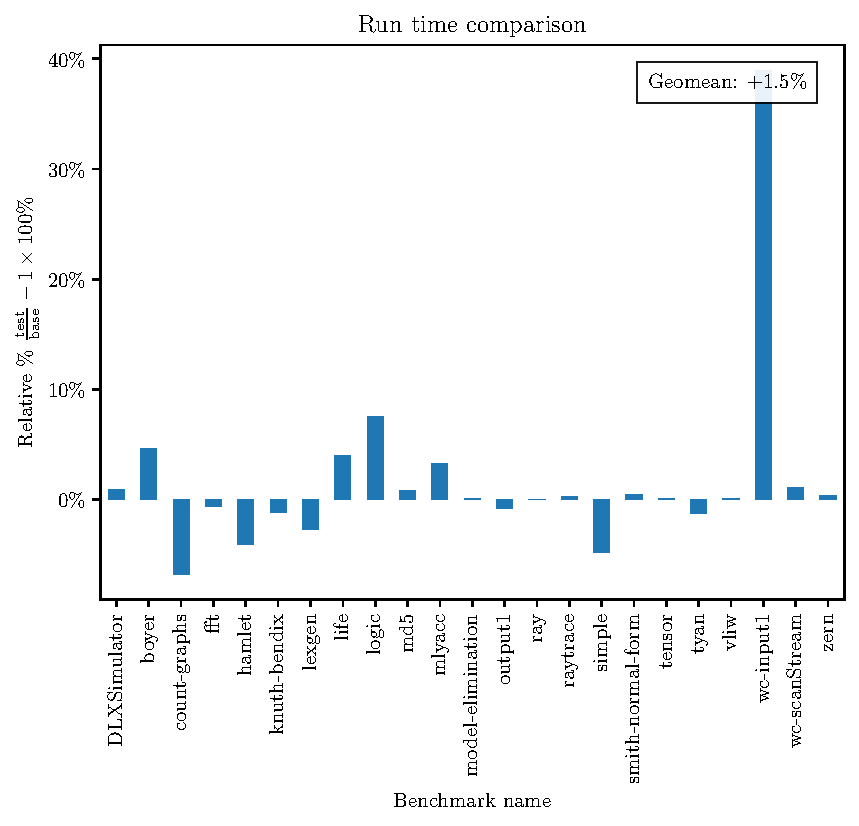
\includegraphics[width=\textwidth]{con_mlton_run_mlton_vs_mlton.pdf}
    \caption{Run time}
    \label{fig:con_mlton_run_mlton_vs_mlton}
  \end{subfigure}
  \hfill
  \begin{subfigure}[b]{0.32\textwidth}
    \centering
    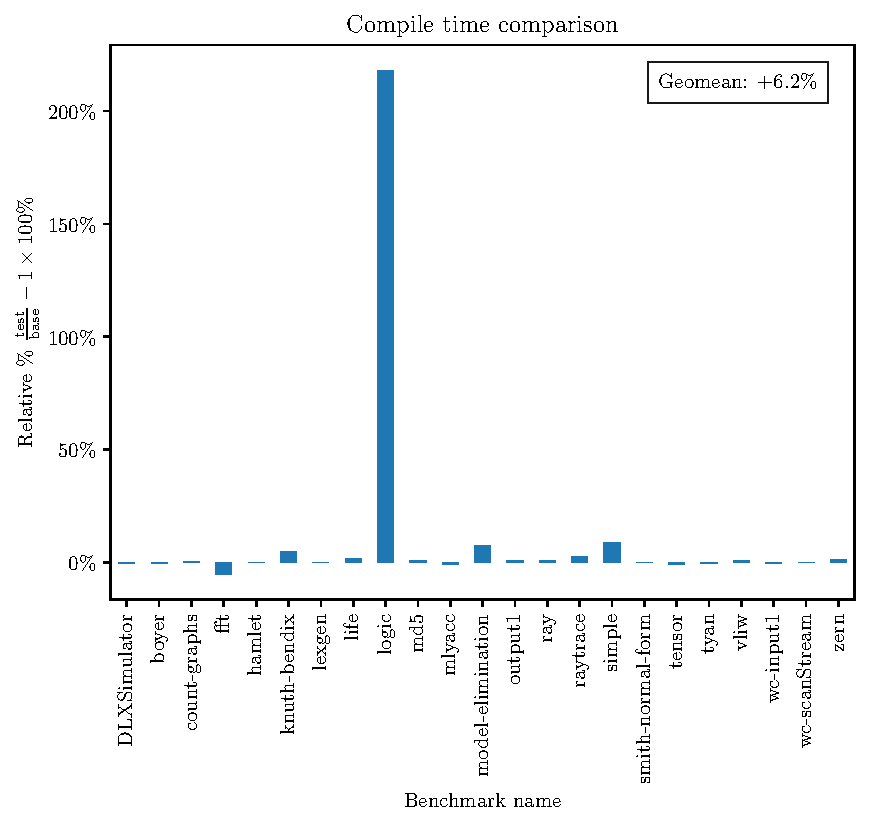
\includegraphics[width=\textwidth]{con_mlton_compile_mlton_vs_mlton.pdf}
    \caption{Compile time}
    \label{fig:con_mlton_compile_mlton_vs_mlton}
  \end{subfigure}
  \hfill
  \begin{subfigure}[b]{0.32\textwidth}
    \centering
    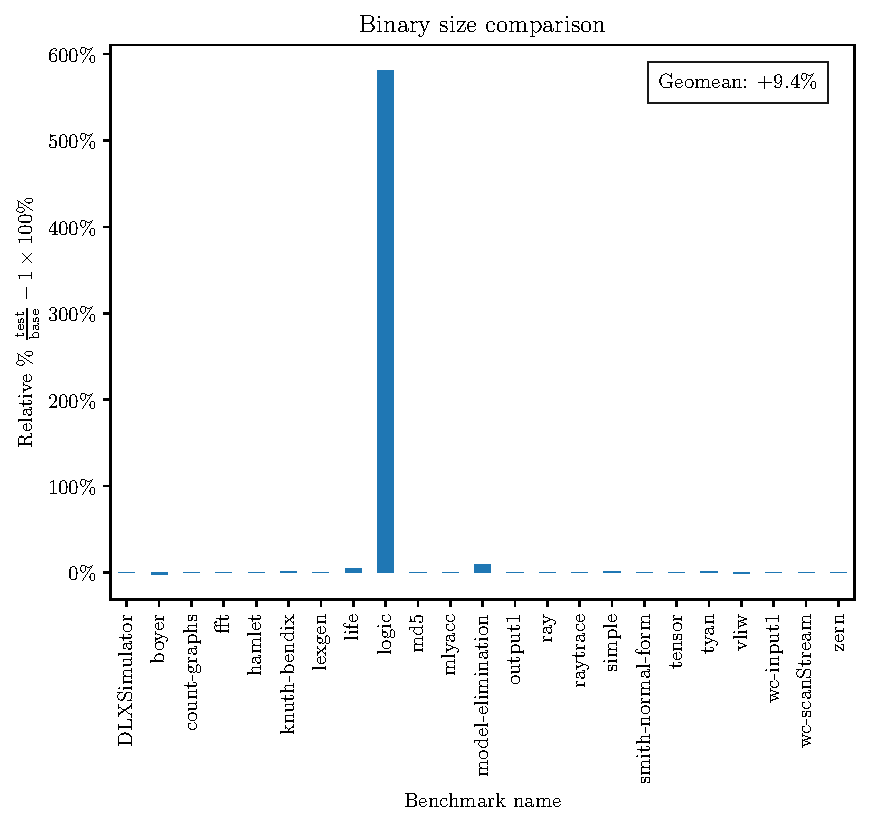
\includegraphics[width=\textwidth]{con_mlton_size_mlton_vs_mlton.pdf}
    \caption{Binary size}
    \label{fig:con_mlton_size_mlton_vs_mlton}
  \end{subfigure}
  \caption{Relative performance for with- vs without-\texttt{PreFlatten}, applied to \texttt{ConApp} on the MLton benchmark suite. Data: \protect\nolinkurl{test_conapp_flatten_mlton_mlton_o3:flattening-tests:fd9a06c:20260825_044217.jsonl}. <0\% represents an improvement, >0\% represents a regression.}
  \label{fig:con_mlton}
\end{figure}

\subsection{\texttt{parallel-ml-bench}: MLton vs MLton (\texttt{ConApp} Flattening)}

\begin{figure}[H]
  \centering
  \begin{subfigure}[b]{0.48\textwidth}
    \centering
    \includegraphics[width=\textwidth]{con_parallel_bench_run_mlton_vs_mlton.pdf}
    \caption{Run time}
    \label{fig:con_parallel_bench_run_mlton_vs_mlton}
  \end{subfigure}
  \hfill
  \begin{subfigure}[b]{0.48\textwidth}
    \centering
    \includegraphics[width=\textwidth]{con_parallel_bench_size_mlton_vs_mlton.pdf}
    \caption{Binary size}
    \label{fig:con_parallel_bench_size_mlton_vs_mlton}
  \end{subfigure}
  \caption{Relative performance for with- vs without-\texttt{PreFlatten}, applied to \texttt{ConApp} on the \texttt{parallel-ml-bench} benchmark suite. Data: \protect\nolinkurl{mlton_con_mlton_parallel_o3:260824-223054:flattening-tests:dcd9cf195eacea093ebe838dcb1d190333218ffd:260824-223054.processed.jsonl}. <0\% represents an improvement, >0\% represents a regression.}
  \label{fig:con_parallel_bench}
\end{figure}

\subsection{\texttt{parallel-ml-bench}: MPL vs MPL (\texttt{ConApp} Flattening)}

\begin{figure}[H]
  \centering
  \begin{subfigure}[b]{0.48\textwidth}
    \centering
    \includegraphics[width=\textwidth]{con_parallel_bench_run_mpl_vs_mpl.pdf}
    \caption{Run time}
    \label{fig:con_parallel_bench_run_mpl_vs_mpl}
  \end{subfigure}
  \hfill
  \begin{subfigure}[b]{0.48\textwidth}
    \centering
    \includegraphics[width=\textwidth]{con_parallel_bench_size_mpl_vs_mpl.pdf}
    \caption{Binary size}
    \label{fig:con_parallel_bench_size_mpl_vs_mpl}
  \end{subfigure}
  \caption{Relative performance for with- vs without-\texttt{PreFlatten}, applied to \texttt{ConApp} on the \texttt{parallel-ml-bench} benchmark suite, for the MPL compiler, at a variety of core counts. Data: \protect\nolinkurl{mpl_con_mpl_parallel_o3_morecores:260825-142321:flattening-tests:475993b514ca4e4f6921a54f390c1ba9bc2350a1:260825-142321.processed.jsonl}. <0\% represents an improvement, >0\% represents a regression.}
  \label{fig:con_parallel_bench_mpl}
\end{figure}

\begin{figure}[H]
  \centering
  \includegraphics[width=\textwidth,height=0.88\textheight,keepaspectratio]{con_parallel_bench_run_mpl_vs_mpl_geomean.pdf}
  \caption{Relative performance for with- vs without-\texttt{PreFlatten}, applied to \texttt{ConApp} on the \texttt{parallel-ml-bench} benchmark suite, for the MPL compiler, at a variety of core counts. Data: \protect\nolinkurl{mpl_con_mpl_parallel_o3_morecores:260825-142321:flattening-tests:475993b514ca4e4f6921a54f390c1ba9bc2350a1:260825-142321.processed.jsonl}. <0\% represents an improvement, >0\% represents a regression.}
  \label{fig:con_parallel_bench_mpl_geomean}
\end{figure}

\begin{figure}[H]
  \centering
  \includegraphics[width=\textwidth,height=0.88\textheight,keepaspectratio]{con_parallel_bench_run_mpl_vs_mpl_trellis.pdf}
  \caption{Relative performance for with- vs without-\texttt{PreFlatten}, applied to \texttt{ConApp} on the \texttt{parallel-ml-bench} benchmark suite, for the MPL compiler, at a variety of core counts. Data: \protect\nolinkurl{mpl_con_mpl_parallel_o3_morecores:260825-142321:flattening-tests:475993b514ca4e4f6921a54f390c1ba9bc2350a1:260825-142321.processed.jsonl}. <0\% represents an improvement, >0\% represents a regression.}
  \label{fig:con_parallel_bench_mpl_trellis}
\end{figure}

\clearpage
\section{AoS Flattening}

\subsection{MLton Benchmarks (AoS Flattening)}

\begin{figure}[H]
  \centering
  \begin{subfigure}[b]{0.32\textwidth}
    \centering
    \includegraphics[width=\textwidth]{aos_mlton_run_mlton_vs_mlton.pdf}
    \caption{Run time}
    \label{fig:aos_mlton_run_mlton_vs_mlton}
  \end{subfigure}
  \hfill
  \begin{subfigure}[b]{0.32\textwidth}
    \centering
    \includegraphics[width=\textwidth]{aos_mlton_compile_mlton_vs_mlton.pdf}
    \caption{Compile time}
    \label{fig:aos_mlton_compile_mlton_vs_mlton}
  \end{subfigure}
  \hfill
  \begin{subfigure}[b]{0.32\textwidth}
    \centering
    \includegraphics[width=\textwidth]{aos_mlton_size_mlton_vs_mlton.pdf}
    \caption{Binary size}
    \label{fig:aos_mlton_size_mlton_vs_mlton}
  \end{subfigure}
  \caption{Relative performance for with- vs without-\texttt{ShallowFlatten}, using the AoS transformation on the MLton benchmark suite. Data: \protect\nolinkurl{test_aos_flatten_mlton_mlton_o3:flattening-tests:fd9a06c:20260825_004326.jsonl}. <0\% represents an improvement, >0\% represents a regression.}
  \label{fig:aos_mlton}
\end{figure}

\subsection{\texttt{parallel-ml-bench}: MLton vs MLton (AoS Flattening)}

\begin{figure}[H]
  \centering
  \begin{subfigure}[b]{0.48\textwidth}
    \centering
    \includegraphics[width=\textwidth]{aos_parallel_bench_run_mlton_vs_mlton.pdf}
    \caption{Run time}
    \label{fig:aos_parallel_bench_run_mlton_vs_mlton}
  \end{subfigure}
  \hfill
  \begin{subfigure}[b]{0.48\textwidth}
    \centering
    \includegraphics[width=\textwidth]{aos_parallel_bench_size_mlton_vs_mlton.pdf}
    \caption{Binary size}
    \label{fig:aos_parallel_bench_size_mlton_vs_mlton}
  \end{subfigure}
  \caption{Relative performance for with- vs without-\texttt{ShallowFlatten}, using the AoS transformation on the \texttt{parallel-ml-bench} benchmark suite. Data: \protect\nolinkurl{mlton_aos_mlton_parallel_o3:260824-220328:flattening-tests:dcd9cf195eacea093ebe838dcb1d190333218ffd:260824-220328.processed.jsonl}. <0\% represents an improvement, >0\% represents a regression.}
  \label{fig:aos_parallel_bench}
\end{figure}

\subsection{\texttt{parallel-ml-bench}: MPL vs MPL (AoS Flattening)}

\begin{figure}[H]
  \centering
  \begin{subfigure}[b]{0.48\textwidth}
    \centering
    \includegraphics[width=\textwidth]{aos_parallel_bench_run_mpl_vs_mpl.pdf}
    \caption{Run time}
    \label{fig:aos_parallel_bench_run_mpl_vs_mpl}
  \end{subfigure}
  \hfill
  \begin{subfigure}[b]{0.48\textwidth}
    \centering
    \includegraphics[width=\textwidth]{aos_parallel_bench_size_mpl_vs_mpl.pdf}
    \caption{Binary size}
    \label{fig:aos_parallel_bench_size_mpl_vs_mpl}
  \end{subfigure}
  \caption{Relative performance for with- vs without-\texttt{ShallowFlatten}, using the AoS transformation on the \texttt{parallel-ml-bench} benchmark suite, for the MPL compiler, at a variety of core counts. Data: \protect\nolinkurl{mpl_aos_mpl_parallel_o3_morecores:260825-125551:flattening-tests:475993b514ca4e4f6921a54f390c1ba9bc2350a1:260825-125551.processed.jsonl}. <0\% represents an improvement, >0\% represents a regression.}
  \label{fig:aos_parallel_bench_mpl}
\end{figure}

\begin{figure}[H]
  \centering
  \includegraphics[width=\textwidth,height=0.88\textheight,keepaspectratio]{aos_parallel_bench_run_mpl_vs_mpl_geomean.pdf}
  \caption{Relative performance for with- vs without-\texttt{ShallowFlatten}, using the AoS transformation on the \texttt{parallel-ml-bench} benchmark suite, for the MPL compiler, at a variety of core counts. Data: \protect\nolinkurl{mpl_aos_mpl_parallel_o3_morecores:260825-125551:flattening-tests:475993b514ca4e4f6921a54f390c1ba9bc2350a1:260825-125551.processed.jsonl}. <0\% represents an improvement, >0\% represents a regression.}
  \label{fig:aos_parallel_bench_mpl_geomean}
\end{figure}

\begin{figure}[H]
  \centering
  \includegraphics[width=\textwidth,height=0.88\textheight,keepaspectratio]{aos_parallel_bench_run_mpl_vs_mpl_trellis.pdf}
  \caption{Relative performance for with- vs without-\texttt{ShallowFlatten}, using the AoS transformation on the \texttt{parallel-ml-bench} benchmark suite, for the MPL compiler, at a variety of core counts. Data: \protect\nolinkurl{mpl_aos_mpl_parallel_o3_morecores:260825-125551:flattening-tests:475993b514ca4e4f6921a54f390c1ba9bc2350a1:260825-125551.processed.jsonl}. <0\% represents an improvement, >0\% represents a regression.}
  \label{fig:aos_parallel_bench_mpl_trellis}
\end{figure}

\clearpage
\section{SoA Flattening}

\subsection{MLton Benchmarks (SoA Flattening)}

\begin{figure}[H]
  \centering
  \begin{subfigure}[b]{0.32\textwidth}
    \centering
    \includegraphics[width=\textwidth]{soa_mlton_run_mlton_vs_mlton.pdf}
    \caption{Run time}
    \label{fig:soa_mlton_run_mlton_vs_mlton}
  \end{subfigure}
  \hfill
  \begin{subfigure}[b]{0.32\textwidth}
    \centering
    \includegraphics[width=\textwidth]{soa_mlton_compile_mlton_vs_mlton.pdf}
    \caption{Compile time}
    \label{fig:soa_mlton_compile_mlton_vs_mlton}
  \end{subfigure}
  \hfill
  \begin{subfigure}[b]{0.32\textwidth}
    \centering
    \includegraphics[width=\textwidth]{soa_mlton_size_mlton_vs_mlton.pdf}
    \caption{Binary size}
    \label{fig:soa_mlton_size_mlton_vs_mlton}
  \end{subfigure}
  \caption{Relative performance for with- vs without-\texttt{ShallowFlatten}, using the SoA transformation on the MLton benchmark suite. Data: \protect\nolinkurl{test_soa_flatten_mlton_mlton_o3:flattening-tests:fd9a06c:20260825_024259.jsonl}. <0\% represents an improvement, >0\% represents a regression.}
  \label{fig:soa_mlton}
\end{figure}

\subsection{\texttt{parallel-ml-bench}: MLton vs MLton (SoA Flattening)}

\begin{figure}[H]
  \centering
  \begin{subfigure}[b]{0.48\textwidth}
    \centering
    \includegraphics[width=\textwidth]{soa_parallel_bench_run_mlton_vs_mlton.pdf}
    \caption{Run time}
    \label{fig:soa_parallel_bench_run_mlton_vs_mlton}
  \end{subfigure}
  \hfill
  \begin{subfigure}[b]{0.48\textwidth}
    \centering
    \includegraphics[width=\textwidth]{soa_parallel_bench_size_mlton_vs_mlton.pdf}
    \caption{Binary size}
    \label{fig:soa_parallel_bench_size_mlton_vs_mlton}
  \end{subfigure}
  \caption{Relative performance for with- vs without-\texttt{ShallowFlatten}, using the SoA transformation on the \texttt{parallel-ml-bench} benchmark suite. Data: \protect\nolinkurl{mlton_soa_mlton_parallel_o3:260824-234803:flattening-tests:dcd9cf195eacea093ebe838dcb1d190333218ffd:260824-234803.processed.jsonl}. <0\% represents an improvement, >0\% represents a regression.}
  \label{fig:soa_parallel_bench}
\end{figure}

\subsection{\texttt{parallel-ml-bench}: MPL vs MPL (SoA Flattening)}

\begin{figure}[H]
  \centering
  \begin{subfigure}[b]{0.48\textwidth}
    \centering
    \includegraphics[width=\textwidth]{soa_parallel_bench_run_mpl_vs_mpl.pdf}
    \caption{Run time}
    \label{fig:soa_parallel_bench_run_mpl_vs_mpl}
  \end{subfigure}
  \hfill
  \begin{subfigure}[b]{0.48\textwidth}
    \centering
    \includegraphics[width=\textwidth]{soa_parallel_bench_size_mpl_vs_mpl.pdf}
    \caption{Binary size}
    \label{fig:soa_parallel_bench_size_mpl_vs_mpl}
  \end{subfigure}
  \caption{Relative performance for with- vs without-\texttt{ShallowFlatten}, using the SoA transformation on the \texttt{parallel-ml-bench} benchmark suite, for the MPL compiler, at a variety of core counts. Data: \protect\nolinkurl{mpl_soa_mpl_parallel_o3_morecores:260825-191404:flattening-tests:475993b514ca4e4f6921a54f390c1ba9bc2350a1:260825-191404.processed.jsonl}. <0\% represents an improvement, >0\% represents a regression.}
  \label{fig:soa_parallel_bench_mpl}
\end{figure}

\begin{figure}[H]
  \centering
  \includegraphics[width=\textwidth,height=0.88\textheight,keepaspectratio]{soa_parallel_bench_run_mpl_vs_mpl_geomean.pdf}
  \caption{Relative performance for with- vs without-\texttt{ShallowFlatten}, using the SoA transformation on the \texttt{parallel-ml-bench} benchmark suite, for the MPL compiler, at a variety of core counts. Data: \protect\nolinkurl{mpl_soa_mpl_parallel_o3_morecores:260825-191404:flattening-tests:475993b514ca4e4f6921a54f390c1ba9bc2350a1:260825-191404.processed.jsonl}. <0\% represents an improvement, >0\% represents a regression.}
  \label{fig:soa_parallel_bench_mpl_geomean}
\end{figure}

\begin{figure}[H]
  \centering
  \includegraphics[width=\textwidth,height=0.88\textheight,keepaspectratio]{soa_parallel_bench_run_mpl_vs_mpl_trellis.pdf}
  \caption{Relative performance for with- vs without-\texttt{ShallowFlatten}, using the SoA transformation on the \texttt{parallel-ml-bench} benchmark suite, for the MPL compiler, at a variety of core counts. Data: \protect\nolinkurl{mpl_soa_mpl_parallel_o3_morecores:260825-191404:flattening-tests:475993b514ca4e4f6921a54f390c1ba9bc2350a1:260825-191404.processed.jsonl}. <0\% represents an improvement, >0\% represents a regression.}
  \label{fig:soa_parallel_bench_mpl_trellis}
\end{figure}

\clearpage
\section{Con Chunkify One Flattening}

\subsection{MLton Benchmarks (Con Chunkify One Flattening)}

\begin{figure}[H]
  \centering
  \begin{subfigure}[b]{0.32\textwidth}
    \centering
    \includegraphics[width=\textwidth]{con_chunkify_one_mlton_run_mlton_vs_mlton.pdf}
    \caption{Run time}
    \label{fig:con_chunkify_one_mlton_run_mlton_vs_mlton}
  \end{subfigure}
  \hfill
  \begin{subfigure}[b]{0.32\textwidth}
    \centering
    \includegraphics[width=\textwidth]{con_chunkify_one_mlton_compile_mlton_vs_mlton.pdf}
    \caption{Compile time}
    \label{fig:con_chunkify_one_mlton_compile_mlton_vs_mlton}
  \end{subfigure}
  \hfill
  \begin{subfigure}[b]{0.32\textwidth}
    \centering
    \includegraphics[width=\textwidth]{con_chunkify_one_mlton_size_mlton_vs_mlton.pdf}
    \caption{Binary size}
    \label{fig:con_chunkify_one_mlton_size_mlton_vs_mlton}
  \end{subfigure}
  \caption{Relative performance for \texttt{con\_chunkify\_one} on the MLton benchmark suite. Data: \protect\nolinkurl{mlton_only_chunkify_one:flattening-tests:5894a329f:20260907_204709.jsonl}. <0\% represents an improvement, >0\% represents a regression.}
  \label{fig:con_chunkify_one_mlton}
\end{figure}

\subsection{\texttt{parallel-ml-bench}: MLton vs MLton (Con Chunkify One Flattening)}

\begin{figure}[H]
  \centering
  \begin{subfigure}[b]{0.48\textwidth}
    \centering
    \includegraphics[width=\textwidth]{con_chunkify_one_parallel_bench_run_mlton_vs_mlton.pdf}
    \caption{Run time}
    \label{fig:con_chunkify_one_parallel_bench_run_mlton_vs_mlton}
  \end{subfigure}
  \hfill
  \begin{subfigure}[b]{0.48\textwidth}
    \centering
    \includegraphics[width=\textwidth]{con_chunkify_one_parallel_bench_size_mlton_vs_mlton.pdf}
    \caption{Binary size}
    \label{fig:con_chunkify_one_parallel_bench_size_mlton_vs_mlton}
  \end{subfigure}
  \caption{Relative performance for \texttt{con\_chunkify\_one} on the \texttt{parallel-ml-bench} benchmark suite. Data: \protect\nolinkurl{mlton_con_vs_con_chunkify_one:260907-185802:flattening-tests:b043c5ca58b04eebc09b15abe9bdf2dacf1ab0f0:260907-185802.processed.jsonl}. <0\% represents an improvement, >0\% represents a regression.}
  \label{fig:con_chunkify_one_parallel_bench}
\end{figure}

\subsection{\texttt{parallel-ml-bench}: MPL vs MPL (Con Chunkify One Flattening)}

\begin{figure}[H]
  \centering
  \begin{subfigure}[b]{0.48\textwidth}
    \centering
    \includegraphics[width=\textwidth]{con_chunkify_one_parallel_bench_run_mpl_vs_mpl.pdf}
    \caption{Run time}
    \label{fig:con_chunkify_one_parallel_bench_run_mpl_vs_mpl}
  \end{subfigure}
  \hfill
  \begin{subfigure}[b]{0.48\textwidth}
    \centering
    \includegraphics[width=\textwidth]{con_chunkify_one_parallel_bench_size_mpl_vs_mpl.pdf}
    \caption{Binary size}
    \label{fig:con_chunkify_one_parallel_bench_size_mpl_vs_mpl}
  \end{subfigure}
  \caption{Relative performance for \texttt{con\_chunkify\_one} on the \texttt{parallel-ml-bench} benchmark suite, for the MPL compiler, at a variety of core counts. Data: \protect\nolinkurl{mpl_con_vs_con_chunkify_one:260906-000633:flattening-tests:c36731376758f74b21aca81e0b86e47af0135308:260906-000633.processed.jsonl}. <0\% represents an improvement, >0\% represents a regression.}
  \label{fig:con_chunkify_one_parallel_bench_mpl}
\end{figure}

\begin{figure}[H]
  \centering
  \includegraphics[width=\textwidth,height=0.88\textheight,keepaspectratio]{con_chunkify_one_parallel_bench_run_mpl_vs_mpl_geomean.pdf}
  \caption{Relative performance for \texttt{con\_chunkify\_one} on the \texttt{parallel-ml-bench} benchmark suite, for the MPL compiler, at a variety of core counts. Data: \protect\nolinkurl{mpl_con_vs_con_chunkify_one:260906-000633:flattening-tests:c36731376758f74b21aca81e0b86e47af0135308:260906-000633.processed.jsonl}. <0\% represents an improvement, >0\% represents a regression.}
  \label{fig:con_chunkify_one_parallel_bench_mpl_geomean}
\end{figure}

\begin{figure}[H]
  \centering
  \includegraphics[width=\textwidth,height=0.88\textheight,keepaspectratio]{con_chunkify_one_parallel_bench_run_mpl_vs_mpl_trellis.pdf}
  \caption{Relative performance for \texttt{con\_chunkify\_one} on the \texttt{parallel-ml-bench} benchmark suite, for the MPL compiler, at a variety of core counts. Data: \protect\nolinkurl{mpl_con_vs_con_chunkify_one:260906-000633:flattening-tests:c36731376758f74b21aca81e0b86e47af0135308:260906-000633.processed.jsonl}. <0\% represents an improvement, >0\% represents a regression.}
  \label{fig:con_chunkify_one_parallel_bench_mpl_trellis}
\end{figure}

\clearpage
\section{Tuple Vs Fixup Flattening}

\subsection{\texttt{parallel-ml-bench}: MPL vs MPL (Tuple Vs Fixup Flattening)}

\begin{figure}[H]
  \centering
  \begin{subfigure}[b]{0.48\textwidth}
    \centering
    \includegraphics[width=\textwidth]{tuple_vs_fixup_parallel_bench_run_mpl_vs_mpl.pdf}
    \caption{Run time}
    \label{fig:tuple_vs_fixup_parallel_bench_run_mpl_vs_mpl}
  \end{subfigure}
  \hfill
  \begin{subfigure}[b]{0.48\textwidth}
    \centering
    \includegraphics[width=\textwidth]{tuple_vs_fixup_parallel_bench_size_mpl_vs_mpl.pdf}
    \caption{Binary size}
    \label{fig:tuple_vs_fixup_parallel_bench_size_mpl_vs_mpl}
  \end{subfigure}
  \caption{Relative performance for \texttt{tuple\_vs\_fixup} on the \texttt{parallel-ml-bench} benchmark suite, for the MPL compiler, at a variety of core counts. Data: \protect\nolinkurl{mpl_tuple_vs_tuple_baseline:260830-201419:flattening-tests:b6534a325456bec8107247d5d4cb0e75f830e988:260830-201419.processed.jsonl}. <0\% represents an improvement, >0\% represents a regression.}
  \label{fig:tuple_vs_fixup_parallel_bench_mpl}
\end{figure}

\begin{figure}[H]
  \centering
  \includegraphics[width=\textwidth,height=0.88\textheight,keepaspectratio]{tuple_vs_fixup_parallel_bench_run_mpl_vs_mpl_geomean.pdf}
  \caption{Relative performance for \texttt{tuple\_vs\_fixup} on the \texttt{parallel-ml-bench} benchmark suite, for the MPL compiler, at a variety of core counts. Data: \protect\nolinkurl{mpl_tuple_vs_tuple_baseline:260830-201419:flattening-tests:b6534a325456bec8107247d5d4cb0e75f830e988:260830-201419.processed.jsonl}. <0\% represents an improvement, >0\% represents a regression.}
  \label{fig:tuple_vs_fixup_parallel_bench_mpl_geomean}
\end{figure}

\begin{figure}[H]
  \centering
  \includegraphics[width=\textwidth,height=0.88\textheight,keepaspectratio]{tuple_vs_fixup_parallel_bench_run_mpl_vs_mpl_trellis.pdf}
  \caption{Relative performance for \texttt{tuple\_vs\_fixup} on the \texttt{parallel-ml-bench} benchmark suite, for the MPL compiler, at a variety of core counts. Data: \protect\nolinkurl{mpl_tuple_vs_tuple_baseline:260830-201419:flattening-tests:b6534a325456bec8107247d5d4cb0e75f830e988:260830-201419.processed.jsonl}. <0\% represents an improvement, >0\% represents a regression.}
  \label{fig:tuple_vs_fixup_parallel_bench_mpl_trellis}
\end{figure}

\clearpage
\section{Tuple Chunkify Func Flattening}

\subsection{\texttt{parallel-ml-bench}: MPL vs MPL (Tuple Chunkify Func Flattening)}

\begin{figure}[H]
  \centering
  \begin{subfigure}[b]{0.48\textwidth}
    \centering
    \includegraphics[width=\textwidth]{tuple_chunkify_func_parallel_bench_run_mpl_vs_mpl.pdf}
    \caption{Run time}
    \label{fig:tuple_chunkify_func_parallel_bench_run_mpl_vs_mpl}
  \end{subfigure}
  \hfill
  \begin{subfigure}[b]{0.48\textwidth}
    \centering
    \includegraphics[width=\textwidth]{tuple_chunkify_func_parallel_bench_size_mpl_vs_mpl.pdf}
    \caption{Binary size}
    \label{fig:tuple_chunkify_func_parallel_bench_size_mpl_vs_mpl}
  \end{subfigure}
  \caption{Relative performance for \texttt{tuple\_chunkify\_func} on the \texttt{parallel-ml-bench} benchmark suite, for the MPL compiler, at a variety of core counts. Data: \protect\nolinkurl{mpl_tuple_vs_tuple_chunkify_func:260831-110020:flattening-tests:0ac21b0883f7a3f6d5c5d768fe100c155bb9274b:260831-110020.processed.jsonl}. <0\% represents an improvement, >0\% represents a regression.}
  \label{fig:tuple_chunkify_func_parallel_bench_mpl}
\end{figure}

\begin{figure}[H]
  \centering
  \includegraphics[width=\textwidth,height=0.88\textheight,keepaspectratio]{tuple_chunkify_func_parallel_bench_run_mpl_vs_mpl_geomean.pdf}
  \caption{Relative performance for \texttt{tuple\_chunkify\_func} on the \texttt{parallel-ml-bench} benchmark suite, for the MPL compiler, at a variety of core counts. Data: \protect\nolinkurl{mpl_tuple_vs_tuple_chunkify_func:260831-110020:flattening-tests:0ac21b0883f7a3f6d5c5d768fe100c155bb9274b:260831-110020.processed.jsonl}. <0\% represents an improvement, >0\% represents a regression.}
  \label{fig:tuple_chunkify_func_parallel_bench_mpl_geomean}
\end{figure}

\begin{figure}[H]
  \centering
  \includegraphics[width=\textwidth,height=0.88\textheight,keepaspectratio]{tuple_chunkify_func_parallel_bench_run_mpl_vs_mpl_trellis.pdf}
  \caption{Relative performance for \texttt{tuple\_chunkify\_func} on the \texttt{parallel-ml-bench} benchmark suite, for the MPL compiler, at a variety of core counts. Data: \protect\nolinkurl{mpl_tuple_vs_tuple_chunkify_func:260831-110020:flattening-tests:0ac21b0883f7a3f6d5c5d768fe100c155bb9274b:260831-110020.processed.jsonl}. <0\% represents an improvement, >0\% represents a regression.}
  \label{fig:tuple_chunkify_func_parallel_bench_mpl_trellis}
\end{figure}

\clearpage
\section{Tuple Chunkify One Flattening}

\subsection{\texttt{parallel-ml-bench}: MPL vs MPL (Tuple Chunkify One Flattening)}

\begin{figure}[H]
  \centering
  \begin{subfigure}[b]{0.48\textwidth}
    \centering
    \includegraphics[width=\textwidth]{tuple_chunkify_one_parallel_bench_run_mpl_vs_mpl.pdf}
    \caption{Run time}
    \label{fig:tuple_chunkify_one_parallel_bench_run_mpl_vs_mpl}
  \end{subfigure}
  \hfill
  \begin{subfigure}[b]{0.48\textwidth}
    \centering
    \includegraphics[width=\textwidth]{tuple_chunkify_one_parallel_bench_size_mpl_vs_mpl.pdf}
    \caption{Binary size}
    \label{fig:tuple_chunkify_one_parallel_bench_size_mpl_vs_mpl}
  \end{subfigure}
  \caption{Relative performance for \texttt{tuple\_chunkify\_one} on the \texttt{parallel-ml-bench} benchmark suite, for the MPL compiler, at a variety of core counts. Data: \protect\nolinkurl{mpl_tuple_vs_tuple_chunkify_one:260901-143537:flattening-tests:2f9a1783de7de96b78f4a934a8afc1d7ebf8c3c6:260901-143537.processed.jsonl}. <0\% represents an improvement, >0\% represents a regression.}
  \label{fig:tuple_chunkify_one_parallel_bench_mpl}
\end{figure}

\begin{figure}[H]
  \centering
  \includegraphics[width=\textwidth,height=0.88\textheight,keepaspectratio]{tuple_chunkify_one_parallel_bench_run_mpl_vs_mpl_geomean.pdf}
  \caption{Relative performance for \texttt{tuple\_chunkify\_one} on the \texttt{parallel-ml-bench} benchmark suite, for the MPL compiler, at a variety of core counts. Data: \protect\nolinkurl{mpl_tuple_vs_tuple_chunkify_one:260901-143537:flattening-tests:2f9a1783de7de96b78f4a934a8afc1d7ebf8c3c6:260901-143537.processed.jsonl}. <0\% represents an improvement, >0\% represents a regression.}
  \label{fig:tuple_chunkify_one_parallel_bench_mpl_geomean}
\end{figure}

\begin{figure}[H]
  \centering
  \includegraphics[width=\textwidth,height=0.88\textheight,keepaspectratio]{tuple_chunkify_one_parallel_bench_run_mpl_vs_mpl_trellis.pdf}
  \caption{Relative performance for \texttt{tuple\_chunkify\_one} on the \texttt{parallel-ml-bench} benchmark suite, for the MPL compiler, at a variety of core counts. Data: \protect\nolinkurl{mpl_tuple_vs_tuple_chunkify_one:260901-143537:flattening-tests:2f9a1783de7de96b78f4a934a8afc1d7ebf8c3c6:260901-143537.processed.jsonl}. <0\% represents an improvement, >0\% represents a regression.}
  \label{fig:tuple_chunkify_one_parallel_bench_mpl_trellis}
\end{figure}

\clearpage
\section{Con Chunkify Func Flattening}

\subsection{\texttt{parallel-ml-bench}: MPL vs MPL (Con Chunkify Func Flattening)}

\begin{figure}[H]
  \centering
  \begin{subfigure}[b]{0.48\textwidth}
    \centering
    \includegraphics[width=\textwidth]{con_chunkify_func_parallel_bench_run_mpl_vs_mpl.pdf}
    \caption{Run time}
    \label{fig:con_chunkify_func_parallel_bench_run_mpl_vs_mpl}
  \end{subfigure}
  \hfill
  \begin{subfigure}[b]{0.48\textwidth}
    \centering
    \includegraphics[width=\textwidth]{con_chunkify_func_parallel_bench_size_mpl_vs_mpl.pdf}
    \caption{Binary size}
    \label{fig:con_chunkify_func_parallel_bench_size_mpl_vs_mpl}
  \end{subfigure}
  \caption{Relative performance for \texttt{con\_chunkify\_func} on the \texttt{parallel-ml-bench} benchmark suite, for the MPL compiler, at a variety of core counts. Data: \protect\nolinkurl{mpl_con_vs_con_chunkify_func:260905-191722:flattening-tests:c36731376758f74b21aca81e0b86e47af0135308:260905-191722.processed.jsonl}. <0\% represents an improvement, >0\% represents a regression.}
  \label{fig:con_chunkify_func_parallel_bench_mpl}
\end{figure}

\begin{figure}[H]
  \centering
  \includegraphics[width=\textwidth,height=0.88\textheight,keepaspectratio]{con_chunkify_func_parallel_bench_run_mpl_vs_mpl_geomean.pdf}
  \caption{Relative performance for \texttt{con\_chunkify\_func} on the \texttt{parallel-ml-bench} benchmark suite, for the MPL compiler, at a variety of core counts. Data: \protect\nolinkurl{mpl_con_vs_con_chunkify_func:260905-191722:flattening-tests:c36731376758f74b21aca81e0b86e47af0135308:260905-191722.processed.jsonl}. <0\% represents an improvement, >0\% represents a regression.}
  \label{fig:con_chunkify_func_parallel_bench_mpl_geomean}
\end{figure}

\begin{figure}[H]
  \centering
  \includegraphics[width=\textwidth,height=0.88\textheight,keepaspectratio]{con_chunkify_func_parallel_bench_run_mpl_vs_mpl_trellis.pdf}
  \caption{Relative performance for \texttt{con\_chunkify\_func} on the \texttt{parallel-ml-bench} benchmark suite, for the MPL compiler, at a variety of core counts. Data: \protect\nolinkurl{mpl_con_vs_con_chunkify_func:260905-191722:flattening-tests:c36731376758f74b21aca81e0b86e47af0135308:260905-191722.processed.jsonl}. <0\% represents an improvement, >0\% represents a regression.}
  \label{fig:con_chunkify_func_parallel_bench_mpl_trellis}
\end{figure}

\clearpage
\section{Aos Chunkify Func Flattening}

\subsection{\texttt{parallel-ml-bench}: MPL vs MPL (Aos Chunkify Func Flattening)}

\begin{figure}[H]
  \centering
  \begin{subfigure}[b]{0.48\textwidth}
    \centering
    \includegraphics[width=\textwidth]{aos_chunkify_func_parallel_bench_run_mpl_vs_mpl.pdf}
    \caption{Run time}
    \label{fig:aos_chunkify_func_parallel_bench_run_mpl_vs_mpl}
  \end{subfigure}
  \hfill
  \begin{subfigure}[b]{0.48\textwidth}
    \centering
    \includegraphics[width=\textwidth]{aos_chunkify_func_parallel_bench_size_mpl_vs_mpl.pdf}
    \caption{Binary size}
    \label{fig:aos_chunkify_func_parallel_bench_size_mpl_vs_mpl}
  \end{subfigure}
  \caption{Relative performance for \texttt{aos\_chunkify\_func} on the \texttt{parallel-ml-bench} benchmark suite, for the MPL compiler, at a variety of core counts. Data: \protect\nolinkurl{mpl_aos_vs_aos_chunkify_func:260908-012113:flattening-tests:ab3558968f943135eaa66e7738b2363ca2b81f71:260908-012113.processed.jsonl}. <0\% represents an improvement, >0\% represents a regression.}
  \label{fig:aos_chunkify_func_parallel_bench_mpl}
\end{figure}

\begin{figure}[H]
  \centering
  \includegraphics[width=\textwidth,height=0.88\textheight,keepaspectratio]{aos_chunkify_func_parallel_bench_run_mpl_vs_mpl_geomean.pdf}
  \caption{Relative performance for \texttt{aos\_chunkify\_func} on the \texttt{parallel-ml-bench} benchmark suite, for the MPL compiler, at a variety of core counts. Data: \protect\nolinkurl{mpl_aos_vs_aos_chunkify_func:260908-012113:flattening-tests:ab3558968f943135eaa66e7738b2363ca2b81f71:260908-012113.processed.jsonl}. <0\% represents an improvement, >0\% represents a regression.}
  \label{fig:aos_chunkify_func_parallel_bench_mpl_geomean}
\end{figure}

\begin{figure}[H]
  \centering
  \includegraphics[width=\textwidth,height=0.88\textheight,keepaspectratio]{aos_chunkify_func_parallel_bench_run_mpl_vs_mpl_trellis.pdf}
  \caption{Relative performance for \texttt{aos\_chunkify\_func} on the \texttt{parallel-ml-bench} benchmark suite, for the MPL compiler, at a variety of core counts. Data: \protect\nolinkurl{mpl_aos_vs_aos_chunkify_func:260908-012113:flattening-tests:ab3558968f943135eaa66e7738b2363ca2b81f71:260908-012113.processed.jsonl}. <0\% represents an improvement, >0\% represents a regression.}
  \label{fig:aos_chunkify_func_parallel_bench_mpl_trellis}
\end{figure}

\clearpage
\section{Aos Chunkify One Flattening}

\subsection{\texttt{parallel-ml-bench}: MPL vs MPL (Aos Chunkify One Flattening)}

\begin{figure}[H]
  \centering
  \begin{subfigure}[b]{0.48\textwidth}
    \centering
    \includegraphics[width=\textwidth]{aos_chunkify_one_parallel_bench_run_mpl_vs_mpl.pdf}
    \caption{Run time}
    \label{fig:aos_chunkify_one_parallel_bench_run_mpl_vs_mpl}
  \end{subfigure}
  \hfill
  \begin{subfigure}[b]{0.48\textwidth}
    \centering
    \includegraphics[width=\textwidth]{aos_chunkify_one_parallel_bench_size_mpl_vs_mpl.pdf}
    \caption{Binary size}
    \label{fig:aos_chunkify_one_parallel_bench_size_mpl_vs_mpl}
  \end{subfigure}
  \caption{Relative performance for \texttt{aos\_chunkify\_one} on the \texttt{parallel-ml-bench} benchmark suite, for the MPL compiler, at a variety of core counts. Data: \protect\nolinkurl{mpl_aos_vs_aos_chunkify_one:260908-025502:flattening-tests:ab3558968f943135eaa66e7738b2363ca2b81f71:260908-025502.processed.jsonl}. <0\% represents an improvement, >0\% represents a regression.}
  \label{fig:aos_chunkify_one_parallel_bench_mpl}
\end{figure}

\begin{figure}[H]
  \centering
  \includegraphics[width=\textwidth,height=0.88\textheight,keepaspectratio]{aos_chunkify_one_parallel_bench_run_mpl_vs_mpl_geomean.pdf}
  \caption{Relative performance for \texttt{aos\_chunkify\_one} on the \texttt{parallel-ml-bench} benchmark suite, for the MPL compiler, at a variety of core counts. Data: \protect\nolinkurl{mpl_aos_vs_aos_chunkify_one:260908-025502:flattening-tests:ab3558968f943135eaa66e7738b2363ca2b81f71:260908-025502.processed.jsonl}. <0\% represents an improvement, >0\% represents a regression.}
  \label{fig:aos_chunkify_one_parallel_bench_mpl_geomean}
\end{figure}

\begin{figure}[H]
  \centering
  \includegraphics[width=\textwidth,height=0.88\textheight,keepaspectratio]{aos_chunkify_one_parallel_bench_run_mpl_vs_mpl_trellis.pdf}
  \caption{Relative performance for \texttt{aos\_chunkify\_one} on the \texttt{parallel-ml-bench} benchmark suite, for the MPL compiler, at a variety of core counts. Data: \protect\nolinkurl{mpl_aos_vs_aos_chunkify_one:260908-025502:flattening-tests:ab3558968f943135eaa66e7738b2363ca2b81f71:260908-025502.processed.jsonl}. <0\% represents an improvement, >0\% represents a regression.}
  \label{fig:aos_chunkify_one_parallel_bench_mpl_trellis}
\end{figure}

\clearpage
\section{Trial Scatter Plots}

\subsection{\texttt{delunay} (\texttt{parallel-ml-bench}: MLton (Tuple Flattening))}

\begin{figure}[H]
  \centering
  \includegraphics[width=\textwidth,keepaspectratio]{delunay_mlton_parallel_ml_bench_scatter.pdf}
  \caption{Per-trial execution times for \texttt{delunay} on the \texttt{parallel-ml-bench} benchmark suite. Data: \protect\nolinkurl{mlton_tuple_mlton_parallel_o3:260825-001542:flattening-tests:dcd9cf195eacea093ebe838dcb1d190333218ffd:260825-001542.processed.jsonl}.}
  \label{fig:delunay_mlton_parallel_ml_bench_scatter}
\end{figure}

\subsection{\texttt{dedup} (\texttt{parallel-ml-bench}: MLton (\texttt{ConApp} Flattening))}

\begin{figure}[H]
  \centering
  \includegraphics[width=\textwidth,keepaspectratio]{dedup_mlton_parallel_ml_bench_scatter.pdf}
  \caption{Per-trial execution times for \texttt{dedup} on the \texttt{parallel-ml-bench} benchmark suite. Data: \protect\nolinkurl{mlton_con_mlton_parallel_o3:260824-223054:flattening-tests:dcd9cf195eacea093ebe838dcb1d190333218ffd:260824-223054.processed.jsonl}.}
  \label{fig:dedup_mlton_parallel_ml_bench_scatter}
\end{figure}

\subsection{\texttt{reverb} (\texttt{parallel-ml-bench}: MLton (Tuple Flattening))}

\begin{figure}[H]
  \centering
  \includegraphics[width=\textwidth,keepaspectratio]{reverb_mlton_parallel_ml_bench_scatter.pdf}
  \caption{Per-trial execution times for \texttt{reverb} on the \texttt{parallel-ml-bench} benchmark suite. Data: \protect\nolinkurl{mlton_tuple_mlton_parallel_o3:260825-001542:flattening-tests:dcd9cf195eacea093ebe838dcb1d190333218ffd:260825-001542.processed.jsonl}.}
  \label{fig:reverb_mlton_parallel_ml_bench_scatter}
\end{figure}

\clearpage
\section{Compare Series}

\subsection{Tuple Exp Geomeans}

\begin{figure}[H]
  \centering
  \includegraphics[width=\textwidth,keepaspectratio]{tuple_exp_geomeans.pdf}
  \caption{Comparison of geometric mean speedups across core counts for \texttt{tuple\_exp\_geomeans}. Data: \protect\nolinkurl{mpl_tuple_mpl_parallel_o3_morecores:260825-204258:flattening-tests:475993b514ca4e4f6921a54f390c1ba9bc2350a1:260825-204258.processed.jsonl}, \protect\nolinkurl{mpl_tuple_vs_tuple_baseline:260830-201419:flattening-tests:b6534a325456bec8107247d5d4cb0e75f830e988:260830-201419.processed.jsonl}, \protect\nolinkurl{mpl_tuple_vs_tuple_chunkify_one:260901-143537:flattening-tests:2f9a1783de7de96b78f4a934a8afc1d7ebf8c3c6:260901-143537.processed.jsonl}. <0\% represents an improvement, >0\% represents a regression.}
  \label{fig:tuple_exp_geomeans}
\end{figure}

\subsection{Tuple Exp Delaunay}

\begin{figure}[H]
  \centering
  \includegraphics[width=\textwidth,keepaspectratio]{tuple_exp_delaunay.pdf}
  \caption{Comparison of \texttt{delaunay} speedups across core counts for \texttt{tuple\_exp\_delaunay}. Data: \protect\nolinkurl{mpl_tuple_mpl_parallel_o3_morecores:260825-204258:flattening-tests:475993b514ca4e4f6921a54f390c1ba9bc2350a1:260825-204258.processed.jsonl}, \protect\nolinkurl{mpl_tuple_vs_tuple_baseline:260830-201419:flattening-tests:b6534a325456bec8107247d5d4cb0e75f830e988:260830-201419.processed.jsonl}, \protect\nolinkurl{mpl_tuple_vs_tuple_chunkify_one:260901-143537:flattening-tests:2f9a1783de7de96b78f4a934a8afc1d7ebf8c3c6:260901-143537.processed.jsonl}. <0\% represents an improvement, >0\% represents a regression.}
  \label{fig:tuple_exp_delaunay}
\end{figure}

\subsection{Tuple Exp Bfs}

\begin{figure}[H]
  \centering
  \includegraphics[width=\textwidth,keepaspectratio]{tuple_exp_bfs.pdf}
  \caption{Comparison of \texttt{bfs} speedups across core counts for \texttt{tuple\_exp\_bfs}. Data: \protect\nolinkurl{mpl_tuple_mpl_parallel_o3_morecores:260825-204258:flattening-tests:475993b514ca4e4f6921a54f390c1ba9bc2350a1:260825-204258.processed.jsonl}, \protect\nolinkurl{mpl_tuple_vs_tuple_baseline:260830-201419:flattening-tests:b6534a325456bec8107247d5d4cb0e75f830e988:260830-201419.processed.jsonl}, \protect\nolinkurl{mpl_tuple_vs_tuple_chunkify_one:260901-143537:flattening-tests:2f9a1783de7de96b78f4a934a8afc1d7ebf8c3c6:260901-143537.processed.jsonl}. <0\% represents an improvement, >0\% represents a regression.}
  \label{fig:tuple_exp_bfs}
\end{figure}

\subsection{Con Exp Suffix Array}

\begin{figure}[H]
  \centering
  \includegraphics[width=\textwidth,keepaspectratio]{con_exp_suffix_array.pdf}
  \caption{Comparison of \texttt{suffix-array} speedups across core counts for \texttt{con\_exp\_suffix\_array}. Data: \protect\nolinkurl{mpl_con_mpl_parallel_o3_morecores:260825-142321:flattening-tests:475993b514ca4e4f6921a54f390c1ba9bc2350a1:260825-142321.processed.jsonl}, \protect\nolinkurl{mpl_con_vs_con_chunkify_one:260906-000633:flattening-tests:c36731376758f74b21aca81e0b86e47af0135308:260906-000633.processed.jsonl}. <0\% represents an improvement, >0\% represents a regression.}
  \label{fig:con_exp_suffix_array}
\end{figure}

\subsection{Con Exp Linearrec}

\begin{figure}[H]
  \centering
  \includegraphics[width=\textwidth,keepaspectratio]{con_exp_linearrec.pdf}
  \caption{Comparison of \texttt{linearrec} speedups across core counts for \texttt{con\_exp\_linearrec}. Data: \protect\nolinkurl{mpl_con_mpl_parallel_o3_morecores:260825-142321:flattening-tests:475993b514ca4e4f6921a54f390c1ba9bc2350a1:260825-142321.processed.jsonl}, \protect\nolinkurl{mpl_con_vs_con_chunkify_one:260906-000633:flattening-tests:c36731376758f74b21aca81e0b86e47af0135308:260906-000633.processed.jsonl}. <0\% represents an improvement, >0\% represents a regression.}
  \label{fig:con_exp_linearrec}
\end{figure}

\subsection{Con Exp Geomean}

\begin{figure}[H]
  \centering
  \includegraphics[width=\textwidth,keepaspectratio]{con_exp_geomean.pdf}
  \caption{Comparison of geometric mean speedups across core counts for \texttt{con\_exp\_geomean}. Data: \protect\nolinkurl{mpl_con_mpl_parallel_o3_morecores:260825-142321:flattening-tests:475993b514ca4e4f6921a54f390c1ba9bc2350a1:260825-142321.processed.jsonl}, \protect\nolinkurl{mpl_con_vs_con_chunkify_one:260906-000633:flattening-tests:c36731376758f74b21aca81e0b86e47af0135308:260906-000633.processed.jsonl}. <0\% represents an improvement, >0\% represents a regression.}
  \label{fig:con_exp_geomean}
\end{figure}

\clearpage
\section{Compare Bar Charts}

\subsection{Mlton Con Chunkify One Parallel Bench}

\begin{figure}[H]
  \centering
  \includegraphics[width=\textwidth,keepaspectratio]{mlton_con_chunkify_one_parallel_bench.pdf}
  \caption{Comparison of benchmark performance for \texttt{mlton\_con\_chunkify\_one\_parallel\_bench} on the \texttt{parallel-ml-bench} benchmark suite. Data: \protect\nolinkurl{mlton_con_mlton_parallel_o3:260824-223054:flattening-tests:dcd9cf195eacea093ebe838dcb1d190333218ffd:260824-223054.processed.jsonl}, \protect\nolinkurl{mlton_con_vs_con_chunkify_one:260907-185802:flattening-tests:b043c5ca58b04eebc09b15abe9bdf2dacf1ab0f0:260907-185802.processed.jsonl}. <0\% represents an improvement, >0\% represents a regression.}
  \label{fig:mlton_con_chunkify_one_parallel_bench}
\end{figure}

\subsection{Mlton Con Chunkify One Mlton Bench}

\begin{figure}[H]
  \centering
  \includegraphics[width=\textwidth,keepaspectratio]{mlton_con_chunkify_one_mlton_bench.pdf}
  \caption{Comparison of benchmark performance for \texttt{mlton\_con\_chunkify\_one\_mlton\_bench} on the MLton benchmark suite. Data: \protect\nolinkurl{test_conapp_flatten_mlton_mlton_o3:flattening-tests:fd9a06c:20260825_044217.jsonl}, \protect\nolinkurl{mlton_only_chunkify_one:flattening-tests:5894a329f:20260907_204709.jsonl}. <0\% represents an improvement, >0\% represents a regression.}
  \label{fig:mlton_con_chunkify_one_mlton_bench}
\end{figure}

\clearpage
\section{Data Tables}

\subsection{Tuple Flattening}

\subsubsection{MLton Benchmarks (Tuple Flattening)}

\paragraph*{Run time}
\importcsv{tuple_mlton_run_mlton_vs_mlton.csv}

\paragraph*{Compile time}
\importcsv{tuple_mlton_compile_mlton_vs_mlton.csv}

\paragraph*{Binary size}
\importcsv{tuple_mlton_size_mlton_vs_mlton.csv}

\subsubsection{\texttt{parallel-ml-bench}: MLton vs MLton (Tuple Flattening)}

\paragraph*{Run time}
\importcsv{tuple_parallel_bench_run_mlton_vs_mlton.csv}

\paragraph*{Binary size}
\importcsv{tuple_parallel_bench_size_mlton_vs_mlton.csv}

\subsubsection{\texttt{parallel-ml-bench}: MPL vs MPL (Tuple Flattening)}

\paragraph*{Run time}
\importcsv{tuple_parallel_bench_run_mpl_vs_mpl.csv}

\paragraph*{Binary size}
\importcsv{tuple_parallel_bench_size_mpl_vs_mpl.csv}

\clearpage
\subsection{\texttt{ConApp} Flattening}

\subsubsection{MLton Benchmarks (\texttt{ConApp} Flattening)}

\paragraph*{Run time}
\importcsv{con_mlton_run_mlton_vs_mlton.csv}

\paragraph*{Compile time}
\importcsv{con_mlton_compile_mlton_vs_mlton.csv}

\paragraph*{Binary size}
\importcsv{con_mlton_size_mlton_vs_mlton.csv}

\subsubsection{\texttt{parallel-ml-bench}: MLton vs MLton (\texttt{ConApp} Flattening)}

\paragraph*{Run time}
\importcsv{con_parallel_bench_run_mlton_vs_mlton.csv}

\paragraph*{Binary size}
\importcsv{con_parallel_bench_size_mlton_vs_mlton.csv}

\subsubsection{\texttt{parallel-ml-bench}: MPL vs MPL (\texttt{ConApp} Flattening)}

\paragraph*{Run time}
\importcsv{con_parallel_bench_run_mpl_vs_mpl.csv}

\paragraph*{Binary size}
\importcsv{con_parallel_bench_size_mpl_vs_mpl.csv}

\clearpage
\subsection{AoS Flattening}

\subsubsection{MLton Benchmarks (AoS Flattening)}

\paragraph*{Run time}
\importcsv{aos_mlton_run_mlton_vs_mlton.csv}

\paragraph*{Compile time}
\importcsv{aos_mlton_compile_mlton_vs_mlton.csv}

\paragraph*{Binary size}
\importcsv{aos_mlton_size_mlton_vs_mlton.csv}

\subsubsection{\texttt{parallel-ml-bench}: MLton vs MLton (AoS Flattening)}

\paragraph*{Run time}
\importcsv{aos_parallel_bench_run_mlton_vs_mlton.csv}

\paragraph*{Binary size}
\importcsv{aos_parallel_bench_size_mlton_vs_mlton.csv}

\subsubsection{\texttt{parallel-ml-bench}: MPL vs MPL (AoS Flattening)}

\paragraph*{Run time}
\importcsv{aos_parallel_bench_run_mpl_vs_mpl.csv}

\paragraph*{Binary size}
\importcsv{aos_parallel_bench_size_mpl_vs_mpl.csv}

\clearpage
\subsection{SoA Flattening}

\subsubsection{MLton Benchmarks (SoA Flattening)}

\paragraph*{Run time}
\importcsv{soa_mlton_run_mlton_vs_mlton.csv}

\paragraph*{Compile time}
\importcsv{soa_mlton_compile_mlton_vs_mlton.csv}

\paragraph*{Binary size}
\importcsv{soa_mlton_size_mlton_vs_mlton.csv}

\subsubsection{\texttt{parallel-ml-bench}: MLton vs MLton (SoA Flattening)}

\paragraph*{Run time}
\importcsv{soa_parallel_bench_run_mlton_vs_mlton.csv}

\paragraph*{Binary size}
\importcsv{soa_parallel_bench_size_mlton_vs_mlton.csv}

\subsubsection{\texttt{parallel-ml-bench}: MPL vs MPL (SoA Flattening)}

\paragraph*{Run time}
\importcsv{soa_parallel_bench_run_mpl_vs_mpl.csv}

\paragraph*{Binary size}
\importcsv{soa_parallel_bench_size_mpl_vs_mpl.csv}

\clearpage
\subsection{Con Chunkify One Flattening}

\subsubsection{MLton Benchmarks (Con Chunkify One Flattening)}

\paragraph*{Run time}
\importcsv{con_chunkify_one_mlton_run_mlton_vs_mlton.csv}

\paragraph*{Compile time}
\importcsv{con_chunkify_one_mlton_compile_mlton_vs_mlton.csv}

\paragraph*{Binary size}
\importcsv{con_chunkify_one_mlton_size_mlton_vs_mlton.csv}

\subsubsection{\texttt{parallel-ml-bench}: MLton vs MLton (Con Chunkify One Flattening)}

\paragraph*{Run time}
\importcsv{con_chunkify_one_parallel_bench_run_mlton_vs_mlton.csv}

\paragraph*{Binary size}
\importcsv{con_chunkify_one_parallel_bench_size_mlton_vs_mlton.csv}

\subsubsection{\texttt{parallel-ml-bench}: MPL vs MPL (Con Chunkify One Flattening)}

\paragraph*{Run time}
\importcsv{con_chunkify_one_parallel_bench_run_mpl_vs_mpl.csv}

\paragraph*{Binary size}
\importcsv{con_chunkify_one_parallel_bench_size_mpl_vs_mpl.csv}

\clearpage
\subsection{Tuple Vs Fixup Flattening}

\subsubsection{\texttt{parallel-ml-bench}: MPL vs MPL (Tuple Vs Fixup Flattening)}

\paragraph*{Run time}
\importcsv{tuple_vs_fixup_parallel_bench_run_mpl_vs_mpl.csv}

\paragraph*{Binary size}
\importcsv{tuple_vs_fixup_parallel_bench_size_mpl_vs_mpl.csv}

\clearpage
\subsection{Tuple Chunkify Func Flattening}

\subsubsection{\texttt{parallel-ml-bench}: MPL vs MPL (Tuple Chunkify Func Flattening)}

\paragraph*{Run time}
\importcsv{tuple_chunkify_func_parallel_bench_run_mpl_vs_mpl.csv}

\paragraph*{Binary size}
\importcsv{tuple_chunkify_func_parallel_bench_size_mpl_vs_mpl.csv}

\clearpage
\subsection{Tuple Chunkify One Flattening}

\subsubsection{\texttt{parallel-ml-bench}: MPL vs MPL (Tuple Chunkify One Flattening)}

\paragraph*{Run time}
\importcsv{tuple_chunkify_one_parallel_bench_run_mpl_vs_mpl.csv}

\paragraph*{Binary size}
\importcsv{tuple_chunkify_one_parallel_bench_size_mpl_vs_mpl.csv}

\clearpage
\subsection{Con Chunkify Func Flattening}

\subsubsection{\texttt{parallel-ml-bench}: MPL vs MPL (Con Chunkify Func Flattening)}

\paragraph*{Run time}
\importcsv{con_chunkify_func_parallel_bench_run_mpl_vs_mpl.csv}

\paragraph*{Binary size}
\importcsv{con_chunkify_func_parallel_bench_size_mpl_vs_mpl.csv}

\clearpage
\subsection{Aos Chunkify Func Flattening}

\subsubsection{\texttt{parallel-ml-bench}: MPL vs MPL (Aos Chunkify Func Flattening)}

\paragraph*{Run time}
\importcsv{aos_chunkify_func_parallel_bench_run_mpl_vs_mpl.csv}

\paragraph*{Binary size}
\importcsv{aos_chunkify_func_parallel_bench_size_mpl_vs_mpl.csv}

\clearpage
\subsection{Aos Chunkify One Flattening}

\subsubsection{\texttt{parallel-ml-bench}: MPL vs MPL (Aos Chunkify One Flattening)}

\paragraph*{Run time}
\importcsv{aos_chunkify_one_parallel_bench_run_mpl_vs_mpl.csv}

\paragraph*{Binary size}
\importcsv{aos_chunkify_one_parallel_bench_size_mpl_vs_mpl.csv}

\clearpage
\subsection{Trial Scatter Plots}

\subsubsection{\texttt{delunay} (\texttt{parallel-ml-bench}: MLton (Tuple Flattening))}

\importcsv{delunay_mlton_parallel_ml_bench_scatter.csv}

\subsubsection{\texttt{dedup} (\texttt{parallel-ml-bench}: MLton (\texttt{ConApp} Flattening))}

\importcsv{dedup_mlton_parallel_ml_bench_scatter.csv}

\subsubsection{\texttt{reverb} (\texttt{parallel-ml-bench}: MLton (Tuple Flattening))}

\importcsv{reverb_mlton_parallel_ml_bench_scatter.csv}

\clearpage
\subsection{Compare Series}

\subsubsection{Tuple Exp Geomeans}

\importcsv{tuple_exp_geomeans.csv}

\subsubsection{Tuple Exp Delaunay}

\importcsv{tuple_exp_delaunay.csv}

\subsubsection{Tuple Exp Bfs}

\importcsv{tuple_exp_bfs.csv}

\subsubsection{Con Exp Suffix Array}

\importcsv{con_exp_suffix_array.csv}

\subsubsection{Con Exp Linearrec}

\importcsv{con_exp_linearrec.csv}

\subsubsection{Con Exp Geomean}

\importcsv{con_exp_geomean.csv}

\clearpage
\subsection{Compare Bar Charts}

\subsubsection{Mlton Con Chunkify One Parallel Bench}

\importcsv{mlton_con_chunkify_one_parallel_bench.csv}

\subsubsection{Mlton Con Chunkify One Mlton Bench}

\importcsv{mlton_con_chunkify_one_mlton_bench.csv}

\end{document}
